\documentclass[12pt,a4paper]{article}
\usepackage[utf8]{inputenc}
\usepackage{amsmath}
\usepackage{amsfonts}
\usepackage{amssymb}
\usepackage{graphicx}
\usepackage{listings}
\author{put your name here}
\title{Analysis of Movie Genre and Critical Reception}
\begin{document}
	\maketitle
	
	\section*{Introduction}
	The dataset {\tt movies.csv} contains 651 observations of different movies across 32 variables. The dataset was edited using the statistical programming language {\tt R} to contain 28 variables, with 6 variables for year, month and day of release at theatres and on DVD collapsed into two date vectors, and other variables coerced to relevant formats (factor for categorical variables, and logical for binary variables). 
	
	\section*{Research Question}
	Do different genres receive varying critical appreciation? It was decided to compare the 5 most prominent movie genres (`Action and Adventure', `Comedy', `Documentary', `Drama', `Mystery and Suspense') with their critical ratings (`Rotten', `Fresh', `Certified Fresh') to determine if there is a statistically significant correlation between the two variables.
	
	\section*{Analysis}
	A preliminary inspection of the data revealed an apparently non-random distribution of critical ratings according to genre. The tables below provide a summary of raw and proportional distributions.
	\begin{figure}
			\begin{verbatim}
	copy and paste here the console output from your raw contingency table
			\end{verbatim}
		\caption{\footnotesize Contingency table}
	\end{figure}
	\begin{figure}
			\begin{verbatim}
                    critics_rating
genre                Rotten Fresh Certified Fresh
  Action & Adventure  0.738 0.138           0.123
  Comedy              0.724 0.161           0.115
  Documentary         0.058 0.615           0.327
  Drama               0.407 0.348           0.246
  Mystery & Suspense  0.492 0.390           0.119
			\end{verbatim}
		\caption{\footnotesize Proportion table along rows}
	\end{figure}

Visualisation of the distribution of the data appears to confirm that certain categories are disproportionately unfavoured by critics.

\begin{figure}[h!]\centering
	\caption{\footnotesize Bar plot}
	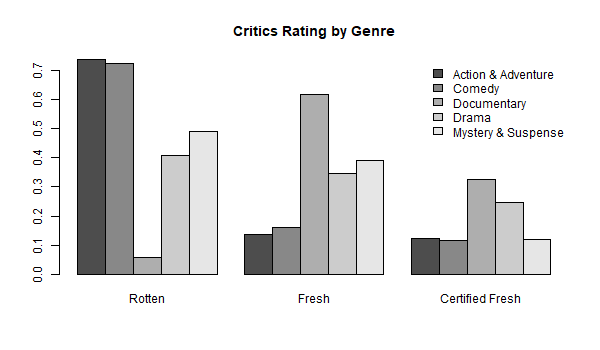
\includegraphics[width=.75\textwidth]{barplot.png}
\end{figure} 

Finally, a statistical test was performed on the data using chi square goodness of fit. The code used is detailed below.

\begin{verbatim}

\lstinputlisting[language=R, firstline=100, lastline=100]{"tutorial03"}
}
The results of the test were as follows:

\begin{verbatim}
	Pearson's Chi-squared test

data:  chi_sq_tbl
X-squared = 86.291, df = 8, p-value = 2.626e-15
\end{verbatim}

\section*{Conclusion}

In conclusion, we rejected the null hypothesis that critical reception is uncorrelated with movie genre. In particular, we note that Action and Adventure and Comedy are statistically more likely to receive rotten reviews, while documentaries are less likely to receive rotten reviews. Residuals are included below.

\begin{verbatim}
copy and paste here the console output from your residuals call
\end{verbatim}

\end{document}